\subsection{Marshallers}

Protokollens hovedfunktionalitet ligger i det der her i systemet kaldes "Marshallers", Hver enkelt kommando klasse har en tilsvarende marshaller der er skræddersyet til at håndtere de attributter der er specifikke for netop den klasse. Derfor skelnes der på samme måde som kommandoer imellem tre typer af marshallers:

\begin{itemize}
	\item \textbf{Generelle marshallers} 
	\item \textbf{Produkt marshallers} 
	\item \textbf{Produktkategori marshallers}
\end{itemize}

Alle tre typer af marshallers implementerer interfacet ICmdMarshaller, og indeholder derfor kun to funktioner.

\begin{itemize}
	\item \textbf{Encode()} 
	\item \textbf{Decode()} 
\end{itemize}

Selve implementeringen af disse funktioner er dog så forskellig at det har været nødvendigt at lave marshallers for hver kommando. Denne design beslutning gav dog også systemet den fordel at det designmæssigt er klart til eventuelle udvidelser uden at skulle ændre i eksisterende funktionalitet og dermed overholder Open-Closed princippet.

\subsubsection{Klassebeskrivelser}
Da UML'en i de forskellige marshallers praktisk talt ligner hinanden er diagrammerne i denne klassebeskrivelse slået sammen til oversigter over de tre typer af marshallers hvortil der vil være en kort beskrivelse af de enkelte klasser.\\

\textbf{Generelle marshallers} håndterer de generelle kommandoer. på figur \ref{fig:overklasseMarsGen} ses en oversigt over de forskellige generelle marshal klasser der alle implementerer ICmdMarshal interfacet.

\begin{figure}[H]
	\centering
	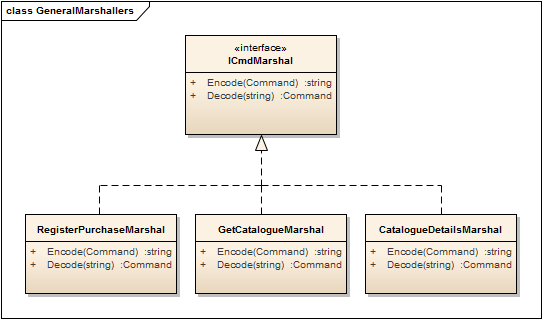
\includegraphics[width=0.8\textwidth]{Systemdesign/SharedLib/Images/Marshallers/GeneralMarshallers2.png}
	\caption{Oversigt over generelle marshallers der nedarver fra ICmdMarshal klassen}
	\label{fig:overklasseMarsGen}
\end{figure}

På figur \ref{fig:overklasseMarsGen} ses først \textit{RegisterPurchaseMarshal}, denne håndterer selvfølgelig RegisterPurchase kommandoen. Dennes encode/decode funktion skal derfor kunne tage højde for et Purchase objekt med en liste af PurchasedProducts og få disse omsat i korrekt format og ligeledes tilbage til de korrekte objekter. 

GetCatalogue kommandoen har i sig selv ingen logik, for yderligere information se figur \ref{fig:klasseCMDGetC}, men dette betyder dog stadig at \textit{GetCatalogueMarshal} skal parse kommando navnet, da det er dette \gls{CS} handler på baggrund af. 

\textit{CatalogueDetailsMarshal} håndterer CatalogueDetails kommandoen og skal derfor kunne parse en liste af ProductCategory objekter der hver især indeholder en liste af Product objekter. Dette gav i første omgang en del problemer da systemet fik indført produktkategorier da det praktisk talt krævede en total revidering af denne klasse.\\


\textbf{Produkt marshallers} håndterer alle de produkt specifikke kommandoer. på figur \ref{fig:overklasseMarsP} ses en oversigt over de forskellige produkt marshal klasser der alle implementerer ICmdMarshal interfacet.

\begin{figure}[H]
	\centering
	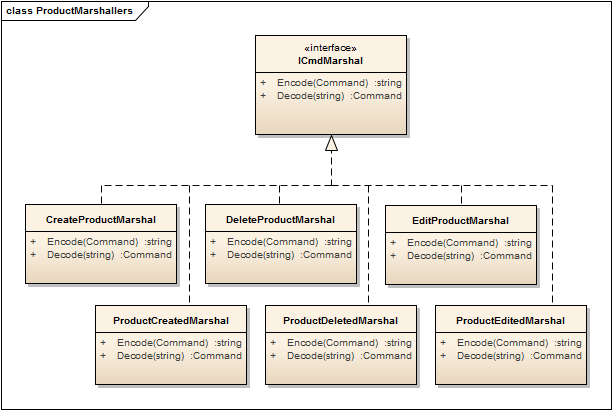
\includegraphics[width=0.8\textwidth]{Systemdesign/SharedLib/Images/Marshallers/ProductMarshallers2.png}
	\caption{Oversigt over produkt specifikke marshallers der implementerer ICmdMarshal interfacet}
	\label{fig:overklasseMarsP}
\end{figure}

På figur \ref{fig:overklasseMarsP} ser den oplyste læser hurtigt at produkt marshallerne på samme måde som kommandoerne kan sættes i par. \textit{CreateProductMarshal} og \textit{ProductCreatedMarshal} håndterer henholdsvis CreateProduct og ProductCreated kommandoerne og skal derfor sørge for at parse Product attributter til og fra XML.

Derefter kommer \textit{DeleteProductMarshal} og \textit{ProductDeletedMarshal} der håndterer henholdsvis DeleteProduct og ProductDeleted kommandoerne, disse skal ligeledes sørge for at parse simple attributter.

Sidst kommer \textit{EditProductMarshal} og \textit{ProductEditedMarshal} der håndterer henholdsvis EditProduct og ProductEdited kommandoerne, disse skal på samme måde som de tidligere marshallers af samme type parse produkt specifikke attributter til og fra XML.\\



\textbf{Produktkategori marshallers} håndterer alle de produktkategori specifikke kommandoer. på figur \ref{fig:overklasseMarsPC} ses en oversigt over de forskellige produktkategori marshal klasser der alle implementerer ICmdMarshal interfacet.

\begin{figure}[H]
	\centering
	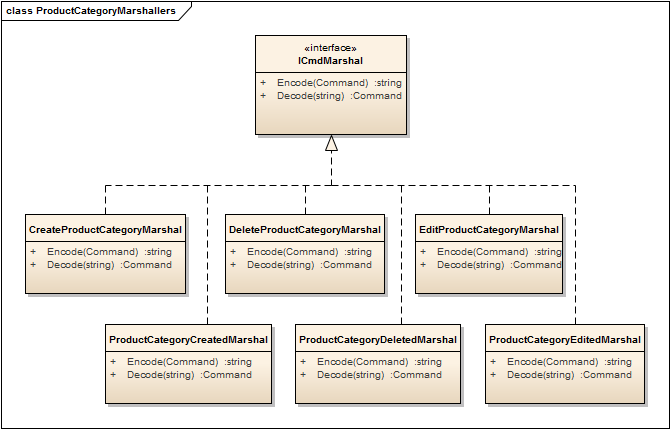
\includegraphics[width=0.8\textwidth]{Systemdesign/SharedLib/Images/Marshallers/ProductCategoryMarshallers2.png}
	\caption{Oversigt over produktkategori specifikke marshallers der nedarver fra ICmdMarshal klassen}
	\label{fig:overklasseMarsPC}
\end{figure}

På figur \ref{fig:overklasseMarsP} ses det meget lignende produkt marshallerne at produktkategori marshallerne på samme måde som kommandoerne kan sættes i par. \textit{CreateProductCategoryMarshal} og \textit{ProductCategoryCreatedMarshal} håndterer henholdsvis CreateProductCategory og ProductCategoryCreated kommandoerne og skal derfor sørge for at parse et ProductCategory objekt med en liste af Product objekter og deres attributter til og fra XML.

Derefter kommer \textit{DeleteProductCategoryMarshal} og \textit{ProductCategoryDeletedMarshal} der håndterer henholdsvis DeleteProductCategory og ProductCategoryDeleted kommandoerne, disse skal ligeledes sørge for at parse et ProductCategory objekt med en liste af Product objekter og deres attributter.

Sidst kommer \textit{EditProductCategoryMarshal} og \textit{ProductCategoryEditedMarshal} der håndterer henholdsvis EditProductCategory og ProductCategoryEdited kommandoerne, disse skal på samme måde som de tidligere marshallers af samme type parse et ProductCategory objekt med en liste af Product objekter og deres attributter til og fra XML.\\



